\section{Zufallsprozess}
Die statistischen Kennwerte sind nun zeitabhängig.
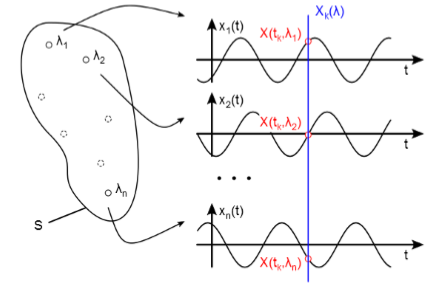
\includegraphics[width=\columnwidth]{Images/zufallsprozess}

\subsection{Stationarität}
Bei stationären Zufallsprozesse ändern sich die statistischen Kennwerte nicht. Mathematisch wird in, wobei jeder SSS auch ein WSS ist.
\begin{enumerate}[nosep]
	\item Wide Sense stationary \textbf{WSS}
	\item Strict sense stationary \textbf{SSS}
\end{enumerate}

Die \textbf{Autokorrelationsfunktion} sagt aus wie ähnlich ein Signal mit sich selber ist: $R_{xx} = E\left[X(t)\cdot X(t+ \tau)\right]$. Die Autokorrelation zum Zeitpunkt 0 entspricht der mittleren Leistung des Signals!

Bei WSS Prozessen gilt der Satz von Plancherel für ein Energiesignal $x_i(t)$
\[
E_i = \int_{-\infty}^{\infty}\left|x_i(t)\right|^2dt \transform \frac{1}{2\pi}\int_{-\infty}^{\infty}\left|X_i(\omega)\right|^2d\omega
\]
Mit der \textbf{Leistungsspektraldichte} $S_{xx}(\omega)$ gilt allgemein:
\[
S_{xx}(\omega) = \lim\limits_{T\rightarrow\infty}E\left[\left|X(\omega)\right|^2\right]
\]
Für WSS Prozesse gilt für $S_{xx}(\omega)$ auch:
\begin{align*}
	S_{xx}(\omega) &= \int_{-\infty}^{\infty}R_{xx}(\tau)e^{-j\omega\tau}d\tau \\
	R_{xx}(\tau) &= \frac{1}{2\pi} \int_{-\infty}^{\infty}S_{xx}(\omega)e^{-j\omega\tau}d\omega
\end{align*}
Eigenschaften:
\begin{itemize}[nosep]
	\item $S_{xx}(-\omega) = S_{xx}(\omega)$
	\item $E\left[X^2(t)\right] = R_{xx}(0) = \frac{1}{2\pi}\int_{-\infty}^{\infty}S_{xx}(\omega)d\omega$
\end{itemize}

\subsubsection{Statische Autokorrelation}\script{169}
\begin{enumerate}[nosep]
	\item Beliebger Punkt $P$ auf $s_{1,2}$ wählen, dieser Amplitudenwert ergibt die $x_k$ Achse
	\item Punkt $P$ um $\tau$ verschieben $P'$
	\item $s_{1+2}$ um $\tau$ verschieben und neu einzeichnen
	\item $P'$ auf verschobenem $s$ ablesen, dieser Amplitudewert ergibt $x_\tau$ Achse
	\item $p_{x_xx_\tau}(x_k,x_\tau)$ ist die Wahrscheinlichkeit des Auftreten der jeweiligen $s$ Funktion. 
	\item Start bei (1), für jede weitere Amplituden Möglichkeit
\end{enumerate}
~\\
\textbf{Tip:} Summe der einzelnen Projektionen auf $x_k$ Achse muss der 1-dimensionaler Amplitudenverteilung entsprechen. ~\\

\noindent\textbf{Beispiel}
\begin{center}
	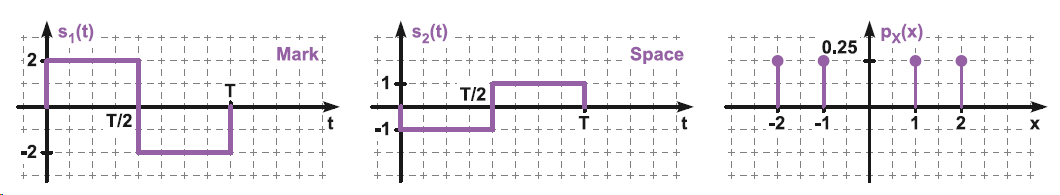
\includegraphics[width=\columnwidth]{Images/statische_ak1}
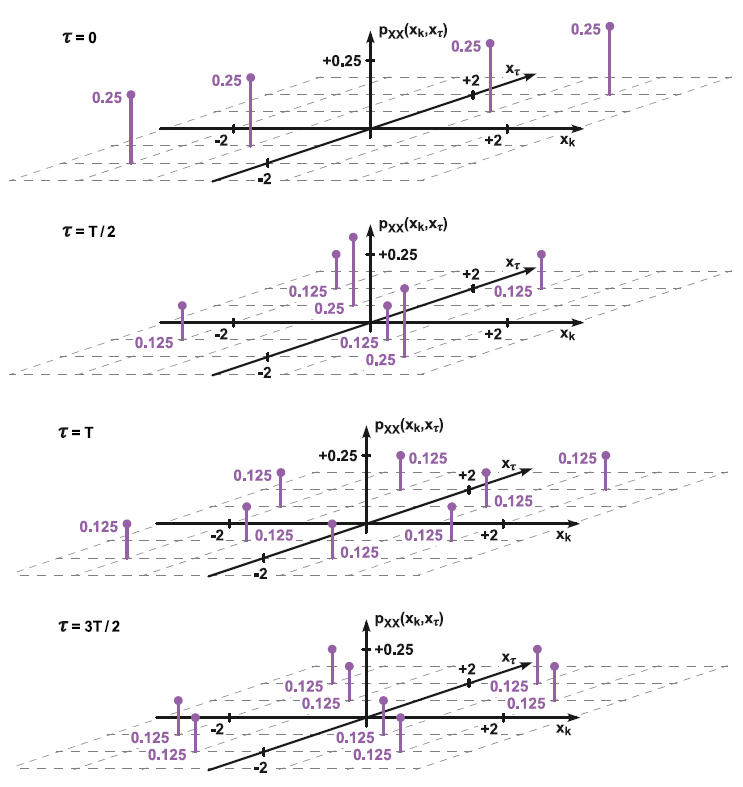
\includegraphics[width=0.8\columnwidth]{Images/statische_ak2}
\end{center}

Daraus lässt sich die Autokorrelationsfunktion $f_{xx}(\tau)$ berechnen:
\begin{align*}
	R_{xx}(\tau = 0) &= 0.25\cdot(-2)^2 + 0.25\cdot (-1)^2+  0.25\cdot(2)^2 + 0.25\cdot (1)^2 \\ &= 2.5 \\
	R_{xx}(\tau = T) &= \sum_{i = 1}^{n}p_i \cdot p_{xx}(x_i) 
\end{align*}

\begin{center}
	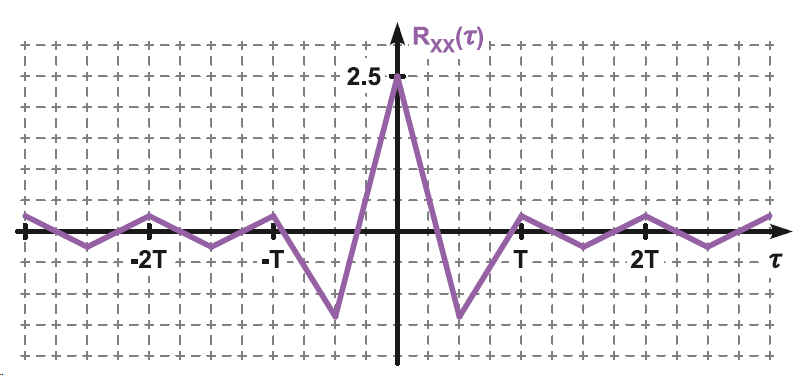
\includegraphics[width=\columnwidth]{Images/statische_ak3}
\end{center}

\subsection{Ergodizität}
Ein stationärer Prozess ist zudem noch ergodisch, wenn alle zeitlichen Mittelwerten (Zeitmittelwert und zeitlich gemittelte Autokorrelation) den statistischen Mittelwerten (Erwartungswert und statistisch gemittelte Autokorrelation) entsprechen. Jeder ergodische Zufallsprozess ist auch stationär, aber nicht umgekehrt.
